% ============================================================
%  S_plan — Final Presentation   KAIST CT-NLP 2026
%  Compile:  pdflatex main.tex  (twice for page numbers)
% ============================================================
\documentclass[aspectratio=169,11pt]{beamer}

% ----- Engine -----------------------------------------------
\usepackage{iftex}
\ifPDFTeX
  \usepackage[scaled=0.93]{helvet}
  \renewcommand{\familydefault}{\sfdefault}
  \usepackage[T1]{fontenc}
  \usepackage[utf8]{inputenc}
\fi

% ----- Packages ---------------------------------------------
\usepackage[table]{xcolor}
\usepackage{booktabs}
\usepackage{amsmath}
\usepackage{graphicx}
\usepackage{tikz}
\usetikzlibrary{positioning,arrows.meta}
\usepackage{tcolorbox}
\tcbuselibrary{most}
\usepackage{array}

% ----- Palette ----------------------------------------------
\definecolor{Navy}{HTML}{1A3055}
\definecolor{Blue}{HTML}{2874A6}
\definecolor{LBlue}{HTML}{D6EAF8}
\definecolor{Green}{HTML}{1A6630}
\definecolor{Red}{HTML}{922B21}
\definecolor{Orange}{HTML}{B9770E}
\definecolor{Muted}{HTML}{717D7E}
\definecolor{HLrow}{HTML}{EBF5FB}

% ----- Theme ------------------------------------------------
\setbeamercolor{background canvas}{bg=white}
\setbeamercolor{normal text}{fg=black}
\setbeamercolor{frametitle}{fg=Navy}
\setbeamercolor{structure}{fg=Blue}
\setbeamertemplate{navigation symbols}{}

\setbeamertemplate{frametitle}{%
  \vspace{0.25cm}%
  {\large\bfseries\color{Navy}\insertframetitle}%
  \ifx\insertframesubtitle\empty\else
    \par\vspace{0.03cm}{\small\color{Muted}\insertframesubtitle}%
  \fi
  \par\vspace{0.05cm}{\color{Blue}\rule{\linewidth}{1.0pt}}\vspace{0.02cm}%
}

\setbeamertemplate{footline}{%
  \leavevmode\hbox{%
    \begin{beamercolorbox}[wd=.75\paperwidth,ht=1.8ex,dp=0.9ex,leftskip=0.4cm]{normal text}%
      \tiny\color{Muted}%
      $S_{\mathrm{plan}}$: Symbolic Planning Tokens for Music-Aware Audio LMs
      \;\textbullet\; KAIST CT-NLP 2026%
    \end{beamercolorbox}%
    \begin{beamercolorbox}[wd=.25\paperwidth,ht=1.8ex,dp=0.9ex,rightskip=0.4cm plus1fil]{normal text}%
      \tiny\color{Muted}\hfill\insertframenumber\,/\,\inserttotalframenumber%
    \end{beamercolorbox}}%
}

\setbeamertemplate{itemize item}{\small\color{Blue}$\blacktriangleright$}
\setlength{\leftmargini}{1.1em}

% ----- Shorthand commands -----------------------------------
\newcommand{\splan}{$S_{\mathrm{plan}}$}
\newcommand{\pos}[1]{{\bfseries\color{Green}#1}}
\newcommand{\bad}[1]{{\color{Red}#1}}
\newcommand{\mute}[1]{{\color{Muted}#1}}
\newcommand{\hook}{$\hookrightarrow$}
\renewcommand{\arraystretch}{1.18}
\setlength{\tabcolsep}{5pt}

% tcolorbox presets  (compact padding)
\tcbset{
  key/.style={colback=LBlue,   colframe=Blue,   boxrule=0.8pt, arc=2pt,
              left=5pt,right=5pt,top=3pt,bottom=3pt, fontupper=\small},
  good/.style={colback=Green!8, colframe=Green,  boxrule=1.0pt, arc=2pt,
              left=5pt,right=5pt,top=3pt,bottom=3pt, fontupper=\small},
  warn/.style={colback=Orange!8,colframe=Orange, boxrule=0.8pt, arc=2pt,
              left=5pt,right=5pt,top=3pt,bottom=3pt, fontupper=\small},
}

% ============================================================
\begin{document}
% ============================================================

% ----------------------------------------------------------------
% 0 — TITLE
% ----------------------------------------------------------------
\begin{frame}[plain]
  \begin{tikzpicture}[remember picture, overlay]
    \fill[Navy] (current page.north west)
                rectangle ([yshift=-4.8cm]current page.north east);
    \node[anchor=north west, inner sep=0pt]
      at ([xshift=0.5cm,yshift=-0.28cm]current page.north west)
      {\tiny\color{LBlue!80}%
       KAIST Graduate School of Cultural Technology\enspace\textbullet\enspace%
       CT-NLP Final Presentation\enspace\textbullet\enspace June 2026};
    \node[anchor=north west,text width=14.5cm,inner sep=0pt]
      at ([xshift=0.5cm,yshift=-0.85cm]current page.north west)
      {\fontsize{17}{21}\selectfont\bfseries\color{white}%
       Toward Symbolic-Aware Music Language Models};
    \node[anchor=north west,text width=13cm,inner sep=0pt]
      at ([xshift=0.5cm,yshift=-1.80cm]current page.north west)
      {\normalsize\color{LBlue}%
       Compact Learned Symbolic Planning Tokens for Controlled Music Fusion};
    \node[anchor=north west,inner sep=0pt]
      at ([xshift=0.5cm,yshift=-2.75cm]current page.north west)
      {\normalsize\color{white!80!Navy}%
       Dabin Kim\quad Minhee Lee\quad Ji Jiaxian\quad Aner Zheng};
    \node[anchor=north west,inner sep=0pt]
      at ([xshift=0.5cm,yshift=-3.35cm]current page.north west)
      {\small\color{LBlue!70}Graduate School of Cultural Technology, KAIST};
  \end{tikzpicture}

  \vspace{5.0cm}
  \begin{tcolorbox}[key]
    Audio language models handle sound well — but musical structure lives in MIDI,
    not in waveforms.
    \textbf{Can we inject symbolic structure into a LALM in a controlled, verifiable way?}
  \end{tcolorbox}
\end{frame}

% ----------------------------------------------------------------
% 1 — PROBLEM
% ----------------------------------------------------------------
\begin{frame}{Audio Tokens Do Not Reliably Encode Musical Structure}

  {\small
  \begin{tabular}{p{5.2cm}p{6.5cm}}
    \toprule
    \textbf{What audio tokens can encode} & \textbf{What they miss} \\
    \midrule
    Timbre, loudness, texture & Key signature, chord progression \\
    General instrument colour & Stem-level instrument identity \\
    Rough tempo feel          & Exact meter and beat phase \\
    High-level scene          & Phrase boundaries, section structure \\
    \bottomrule
  \end{tabular}}

  \smallskip
  MIDI encodes these exactly: note events, instrument tracks, tempo and key events.
  We learn a \emph{compact} representation of this information and inject it into a LALM.

  \smallskip
  \begin{tcolorbox}[key]
    Verifying that symbolic injection is \emph{useful} requires more than comparing to
    no-injection: a shuffled or dummy stream of the same length could produce the same
    gain from capacity alone.
    \textbf{Our whole evaluation is designed around this distinction.}
  \end{tcolorbox}
\end{frame}

% ----------------------------------------------------------------
% 2 — RESEARCH QUESTIONS
% ----------------------------------------------------------------
\begin{frame}{Three Research Questions Organize This Work}

  {\small
  \begin{tabular}{p{2.2cm}p{10.0cm}}
    \toprule
    \textbf{Question} & \textbf{What we need to show} \\
    \midrule
    \textbf{RQ1}\\Acoustic utility &
      Aligned symbolic stream reduces acoustic token cross-entropy more than a shuffled
      or dummy stream of the same size. \\[8pt]
    \textbf{RQ2}\\Alignment specificity &
      The gain comes from \emph{alignment-specific content}, not token budget or
      model capacity.  Requires aligned $>$ shuffled AND aligned $>$ dummy. \\[8pt]
    \textbf{RQ3}\\Structural content &
      Symbolic stream encodes music-structural attributes recoverable by probing —
      verified against a zero-feature baseline that exposes dataset priors. \\
    \bottomrule
  \end{tabular}}

  \smallskip
  \begin{tcolorbox}[key]
    Experiments are \textbf{evidence for these claims}, not the claims themselves.
    Each comparison uses the same aligned / shuffled / dummy protocol so gains can be
    attributed precisely to symbolic content — not to extra tokens.
  \end{tcolorbox}
\end{frame}

% ----------------------------------------------------------------
% 3 — APPROACH
% ----------------------------------------------------------------
\begin{frame}{Our Approach: \splan{} as a Third Stream in UniAudio 2.0}

  \begin{center}
  \vspace{0.3cm}
  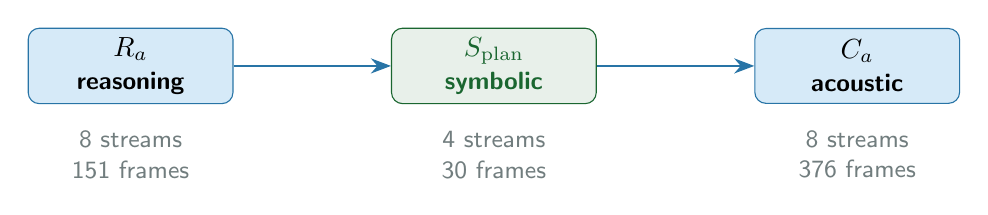
\begin{tikzpicture}[
    box/.style={draw=Blue,fill=LBlue,rounded corners=4pt,
                minimum height=0.95cm,minimum width=2.6cm,
                font=\bfseries\normalsize,align=center},
    newbox/.style={draw=Green,fill=Green!10,rounded corners=4pt,
                   minimum height=0.95cm,minimum width=2.6cm,
                   font=\bfseries\normalsize\color{Green},align=center},
    arr/.style={-{Stealth[scale=1.1]},thick,color=Blue},
    lbl/.style={font=\small\color{Muted},align=center}
  ]
    \node[box]    (ra) {$R_a$\\{\small reasoning}};
    \node[newbox, right=2.0cm of ra] (sp) {\splan{}\\{\small symbolic}};
    \node[box,    right=2.0cm of sp] (ca) {$C_a$\\{\small acoustic}};
    \draw[arr] (ra) -- (sp);
    \draw[arr] (sp) -- (ca);
    \node[lbl,below=0.22cm of ra] {8 streams\\151 frames};
    \node[lbl,below=0.22cm of sp] {4 streams\\30 frames};
    \node[lbl,below=0.22cm of ca] {8 streams\\376 frames};
  \end{tikzpicture}
  \end{center}

  \smallskip
  \splan{} uses a 4-stage RVQ codec trained on MIDI-derived frame features
  (pitch-class, instrument, meter, density).
  Total sequence: $151 + 30 + 376 = \mathbf{557}$ tokens — \textbf{0\% truncation} under 1{,}024 limit.

  \smallskip
  \begin{tcolorbox}[key]
    Raw MIDI appending fails: 2{,}000–8{,}000 tokens per window saturates the context,
    and variable-length sequences cannot be shuffled or dummy-controlled uniformly.
    \splan{}'s fixed-length RVQ design makes the evaluation protocol possible.
  \end{tcolorbox}
\end{frame}

% ----------------------------------------------------------------
% 4 — CONTROLS
% ----------------------------------------------------------------
\begin{frame}{Evaluation Protocol: Every Comparison Uses All Four Conditions}
  \framesubtitle{A gain of aligned over both shuffled and dummy is required for an alignment-specific claim}

  {\small
  \begin{tabular}{p{3.0cm}p{4.5cm}p{4.5cm}}
    \toprule
    \textbf{Condition} & \textbf{Content of \splan{} slot} &
      \textbf{What a gain here proves} \\
    \midrule
    Aligned \splan{}  & Tokens from the \emph{same} window's MIDI &
      Symbolic content + temporal alignment \\[4pt]
    Shuffled \splan{} & Tokens from a \emph{different} window's MIDI &
      Token statistics intact; alignment broken \\[4pt]
    Dummy stream      & Zero / random RVQ codes &
      Token-budget / capacity effect only \\[4pt]
    Reason-only       & No \splan{} slot at all &
      Base model without any symbolic stream \\
    \bottomrule
  \end{tabular}}

  \smallskip
  \begin{tcolorbox}[good]
    \textbf{Claim rule:} aligned must beat \emph{both} shuffled and dummy.
    Shuffled preserves statistics but breaks alignment; dummy removes all content.
    Together they isolate the alignment-specific effect from pure capacity.
  \end{tcolorbox}
\end{frame}

% ----------------------------------------------------------------
% 5 — PREREQUISITE: CODEC TABLE
% ----------------------------------------------------------------
\begin{frame}{Prerequisite: The Symbolic Codec Reconstructs Faithfully}
  \framesubtitle{4-stage RVQ, 512 codes per stage — 42{,}000 training steps on Slakh}

  {\small
  \begin{tabular}{ll}
    \toprule
    \textbf{Metric} & \textbf{Value} \\
    \midrule
    Validation reconstruction loss              & 0.00918 \\
    Binary feature accuracy                     & \pos{0.99777} \\
    Continuous feature MSE                      & \pos{0.00172} \\
    Codebook utilization — books 1/2/3/4        & 31\% / 72\% / 81\% / 81\% \\
    \midrule
    Fixed window \texttt{w000} binary acc / MSE & 1.000 / 0.00174 \\
    Fixed window \texttt{w001} binary acc / MSE & 1.000 / 0.00246 \\
    Fixed window \texttt{w003} binary acc / MSE & 1.000 / 0.00130 \\
    \bottomrule
  \end{tabular}}

  \smallskip
  \begin{tcolorbox}[good]
    Books 2–4 reach 72–81\% utilization — no codebook collapse.
    This is a \textbf{prerequisite}, not a claim: it establishes that
    differences in downstream comparisons come from symbolic content, not codec failure.
  \end{tcolorbox}
\end{frame}

% ----------------------------------------------------------------
% 6 — PREREQUISITE: CODEC FIGURE
% ----------------------------------------------------------------
\begin{frame}{Prerequisite: Feature Heatmap — Target vs.\ Reconstruction}
  \framesubtitle{Slakh Track01501, window 0 (0–30 s) — binary acc 1.000, MSE 0.00174}

  \begin{center}
    \includegraphics[width=\textwidth,height=0.58\textheight,keepaspectratio]%
      {splan_recon_track01501_w000_s0000000_feature_heatmap.png}
  \end{center}

  \smallskip
  {\footnotesize\color{Muted}%
   Rows: feature dimensions (binary instrument flags, pitch-class bits, continuous values).
   Columns: 30 time frames (1\,s each).
   Left = ground-truth MIDI features. Right = \splan{} reconstruction.}
\end{frame}

% ----------------------------------------------------------------
% 7 — RQ1: PROXY TASK
% ----------------------------------------------------------------
\begin{frame}{RQ1 — First Positive Signal: Proxy Prediction Task}
  \framesubtitle{Frozen codec + small transformer head predicting acoustic tokens from symbolic representations}

  {\small
  \begin{tabular}{p{4.0cm}ccc}
    \toprule
    \textbf{Condition} & \textbf{Valid CE} & \textbf{Test CE} & \textbf{Test PPL} \\
    \midrule
    Reason only            & 7.565 & 7.657 & 2116 \\
    Low-rate rule summary  & 7.553 & 7.645 & 2089 \\
    \rowcolor{HLrow}
    \textbf{Aligned \splan{}} & \textbf{7.507} & \textbf{7.596} & \textbf{1991} \\
    \hook{} Shuffled \splan{} & 7.538 & 7.631 & 2061 \\
    \hook{} Dummy stream      & 7.602 & 7.694 & 2196 \\
    \hook{} Random stream     & 7.540 & 7.632 & 2064 \\
    \bottomrule
  \end{tabular}}

  \smallskip
  Aligned beats reason-only ($\Delta{=}{-}0.061$) and shuffled ($\Delta{=}{-}0.034$).
  Learned \splan{} outperforms the hand-crafted rule summary ($-0.048$ vs.\ $-0.013$).

  \smallskip
  \begin{tcolorbox}[good]
    \textbf{First evidence for RQ1.} Aligned beats both corrupted controls.
    Temporal alignment of symbolic content to its own audio window drives the gain.
    Claim boundary: proxy task; end-to-end integration is tested separately.
  \end{tcolorbox}
\end{frame}

% ----------------------------------------------------------------
% 8 — RQ1: STREAM-NATIVE
% ----------------------------------------------------------------
\begin{frame}{RQ1 — Replication: Stream-Native Interface Confirms the Gain}
  \framesubtitle{Full $R_a \to S_{\mathrm{plan}} \to C_a$ layout with matched positional encoding}

  {\small
  \begin{tabular}{p{4.0cm}ccc}
    \toprule
    \textbf{Condition} & \textbf{Test CE} & \textbf{Test Acc} & \textbf{Gate} \\
    \midrule
    \rowcolor{HLrow}
    Aligned \splan{}  & \textbf{5.766} & \textbf{0.1097} & 0.003 \\
    \hook{} Shuffled  & 5.785 & 0.1067 & 0.003 \\
    \hook{} Dummy     & 5.785 & 0.1068 & 0.003 \\
    \bottomrule
  \end{tabular}}

  \smallskip
  Aligned beats shuffled ($\Delta{=}{-}0.018$) and dummy ($\Delta{=}{-}0.019$) consistently.
  Sequence 557 tokens, \textbf{0\% truncation}.

  \smallskip
  \begin{tcolorbox}[good]
    \textbf{RQ1 holds with end-to-end integration.}
    The positive gap replicates when \splan{} is inserted as a native third stream —
    not just as an external side-channel.
    This rules out a proxy-task artifact.
  \end{tcolorbox}
\end{frame}

% ----------------------------------------------------------------
% 9 — RQ1: PRIMARY RESULT
% ----------------------------------------------------------------
\begin{frame}{RQ1 — Primary Result: Hardened Four-Condition Comparison}
  \framesubtitle{All four conditions identical except stream variant — matched hyperparameters, fixed seed}

  {\small
  \begin{tabular}{p{4.0cm}cccc}
    \toprule
    \textbf{Condition} & \textbf{Test CE} & \textbf{Test PPL} & \textbf{Acc} & \textbf{Gate} \\
    \midrule
    Reason-only baseline    & 5.859 & 350 & 0.104 & 0.000 \\
    \rowcolor{HLrow}
    \textbf{Aligned \splan{}} & \textbf{5.600} & \textbf{270} & \textbf{0.121} & \textbf{0.177} \\
    \hook{} Shuffled \splan{} & 5.614 & 274 & 0.119 & 0.167 \\
    \hook{} Dummy stream      & 5.614 & 274 & 0.119 & 0.163 \\
    \bottomrule
  \end{tabular}}

  \smallskip
  Aligned beats both corrupted controls ($\Delta{=}{-}0.014$) on top of a large
  capacity gain ($-0.245$ vs.\ reason-only).

  \smallskip
  \begin{tcolorbox}[good]
    \textbf{RQ1 answered positively} — most rigorous evidence.
    Gate confirms the model opens the symbolic slot more for aligned (0.177)
    than shuffled (0.167) or dummy (0.163).\\
    Boundary: oracle MIDI input; semantic-token CE only.
  \end{tcolorbox}
\end{frame}

% ----------------------------------------------------------------
% 10 — RQ2: DECOMPOSITION + CONSISTENCY
% ----------------------------------------------------------------
\begin{frame}{RQ2: The Gain Is Alignment-Specific, Not Token Capacity}

  The $-0.259$ CE gain over reason-only decomposes into two distinct effects:

  {\small
  \begin{tabular}{p{8.0cm}c}
    \toprule
    \textbf{Effect} & \textbf{$\Delta$ CE} \\
    \midrule
    Stream capacity (any symbolic stream vs.\ reason-only) & $-0.245$ \\
    Alignment-specific (aligned vs.\ both controls)        & $-0.014$ \\
    \midrule
    \textbf{Total (aligned vs.\ reason-only)} & $\mathbf{-0.259}$ \\
    \bottomrule
  \end{tabular}}

  \smallskip
  The alignment-specific effect is consistent across all three controlled comparisons:

  {\small
  \begin{tabular}{p{4.5cm}p{4.0cm}c}
    \toprule
    \textbf{Comparison} & \textbf{Setup} & \textbf{Aligned vs.\ shuffled} \\
    \midrule
    Proxy task          & Frozen codec, 5{,}000 steps   & $-0.034$ \\
    Stream-native warmup & End-to-end, 3{,}000 steps    & $-0.018$ \\
    Hardened comparison & Matched, 800 steps            & $-0.014$ \\
    \bottomrule
  \end{tabular}}

  \smallskip
  \begin{tcolorbox}[good]
    \textbf{RQ2 answered positively.} Consistent direction across independent setups rules
    out a single-run artifact. Capacity effect is dominant; alignment-specific effect is
    smaller but robust — and corroborated by the gate signal.
  \end{tcolorbox}
\end{frame}

% ----------------------------------------------------------------
% 11 — RQ3: MIR PROBING
% ----------------------------------------------------------------
\begin{frame}{RQ3: Music Structure Is Recoverable from \splan{}}
  \framesubtitle{Supervised probing on frozen embeddings vs.\ zero-feature baseline (head bias only)}

  {\small
  \begin{tabular}{p{4.0cm}cc}
    \toprule
    \textbf{MIR attribute} & \textbf{Aligned \splan{}} & \textbf{Zero-feature control} \\
    \midrule
    Weak key accuracy     & \pos{0.557} & 0.126 \\
    Pitch-class macro-F1  & \pos{0.854} & 0.830 \\
    Instrument macro-F1   & \pos{0.501} & 0.426 \\
    Segment density acc.  & 0.874       & 0.879 \\
    \midrule
    Instrument micro-F1   & 0.791 & \bad{0.835} \\
    Meter accuracy        & 0.783 & \bad{0.855} \\
    \bottomrule
  \end{tabular}}

  \mute{\footnotesize Red = zero-feature control outperforms — these axes are prior-dominated.}

  \smallskip
  \begin{tcolorbox}[key]
    High accuracy alone is \emph{not} evidence — a zero-feature baseline is mandatory.
    Weak key ($+0.431$ gap) and pitch-class ($+0.024$ gap) are the strongest safe axes.
    \textbf{RQ3: qualified positive answer} — key and pitch-class confirmed, meter and
    instrument micro-F1 excluded.
  \end{tcolorbox}
\end{frame}

% ----------------------------------------------------------------
% 12 — RQ3: AXIS SAFETY
% ----------------------------------------------------------------
\begin{frame}{RQ3: Which Axes Can We Claim?}
  \framesubtitle{Organized by what the zero-feature control reveals about each attribute}

  {\small
  \begin{tabular}{p{3.0cm}p{2.5cm}p{6.2cm}}
    \toprule
    \textbf{Axis} & \textbf{Gap vs.\ zero-feat.} & \textbf{Status} \\
    \midrule
    Weak key accuracy     & $+0.431$ & \pos{Safe to claim.} Label-shuffle control pending. \\
    Pitch-class macro-F1  & $+0.024$ & Positive but small; target-prior control needed. \\
    Instrument macro-F1   & $+0.075$ & Some signal; class imbalance must be resolved. \\
    \midrule
    Instrument micro-F1   & $-0.044$ & \bad{Excluded.} Common-class prior dominates. \\
    Meter accuracy        & $-0.072$ & \bad{Excluded.} Common-meter prior dominates. \\
    \bottomrule
  \end{tabular}}

  \smallskip
  \begin{tcolorbox}[warn]
    Paper-safe claim: weak key, pitch-class, and instrument macro-F1 — always reported
    \emph{alongside} the zero-feature gap, not as standalone numbers.
    Label-shuffle and target-prior controls are pending.
  \end{tcolorbox}
\end{frame}

% ----------------------------------------------------------------
% 13 — RQ3: QUALITATIVE FIGURE
% ----------------------------------------------------------------
\begin{frame}{RQ3: Qualitative — Reconstruction vs.\ Ground-Truth Piano Roll}
  \framesubtitle{Slakh Track01501, window 3 (90–120 s) — binary acc 1.000, MSE 0.00130}

  \begin{center}
    \includegraphics[width=\textwidth,height=0.58\textheight,keepaspectratio]%
      {splan_recon_track01501_w003_s0009000_roll_comparison.png}
  \end{center}

  \smallskip
  {\footnotesize\color{Muted}%
   Left: ground-truth MIDI piano roll.\quad
   Right: pitch-region reconstruction from the \splan{} codec.\\
   Boundary: symbolic feature reconstruction — not MIDI transcription or waveform generation.}
\end{frame}

% ----------------------------------------------------------------
% 14 — DESIGN CONSTRAINT
% ----------------------------------------------------------------
\begin{frame}{Design Constraint: Stream-Native Interface Is Necessary}
  \framesubtitle{Two negative results that establish the interface requirement — not incidental failures}

  \textbf{Side-channel insertion:}

  {\small
  \begin{tabular}{p{4.5cm}cc}
    \toprule
    \textbf{Condition} & \textbf{Test CE} & \textbf{vs.\ reason-only} \\
    \midrule
    Reason-only          & \pos{5.360} & baseline \\
    Aligned \splan{}     & 5.511 & \bad{$+0.151$} \\
    Shuffled \splan{}    & 5.512 & \bad{$+0.152$} \\
    Dummy                & 5.510 & \bad{$+0.150$} \\
    \bottomrule
  \end{tabular}}

  \smallskip
  Aligned $\approx$ shuffled $\approx$ dummy: model ignores symbolic content entirely.
  \textbf{Adapter gating:} gate converges to $3.4\times10^{-4}$ — training stable, fusion absent.

  \smallskip
  \begin{tcolorbox}[warn]
    Same root cause in both cases: symbolic tokens must enter through the same stream-native
    positional encoding as $R_a$ and $C_a$.
    \textbf{This is why the RQ1/RQ2 positive results are non-trivial.}
  \end{tcolorbox}
\end{frame}

% ----------------------------------------------------------------
% 15 — LIMITATIONS
% ----------------------------------------------------------------
\begin{frame}{What We Cannot Claim Yet}

  {\small
  \begin{tabular}{p{3.0cm}p{9.0cm}}
    \toprule
    \textbf{Gap} & \textbf{Why it matters} \\
    \midrule
    No decoded generation &
      CE results are on semantic tokens only. No waveform decoded from aligned vs.\ shuffled. \\[4pt]
    Oracle MIDI input &
      Aligned MIDI unavailable at inference on real audio. Needs audio-to-\splan{} predictor. \\[4pt]
    No LLM-supervised tokenizer &
      Text-language grounding (open QA, captioning) not yet trained. \\[4pt]
    Pending MIR controls &
      Label-shuffle and target-prior controls for probing are incomplete. \\[4pt]
    Slakh only &
      No real-recording or cross-domain transfer evidence. \\
    \bottomrule
  \end{tabular}}

  \smallskip
  \begin{tcolorbox}[warn]
    \textbf{Next priority:} decode $C_a$ from the aligned checkpoint to waveform and
    compare perceptually against shuffled — converting the token-level claim into
    perceptual audio evidence.
  \end{tcolorbox}
\end{frame}

% ----------------------------------------------------------------
% 16 — CONCLUSION
% ----------------------------------------------------------------
\begin{frame}{Conclusion: Three Research Questions Answered}

  {\small
  \begin{tabular}{p{1.5cm}p{10.5cm}}
    \toprule
    \textbf{RQ} & \textbf{Finding} \\
    \midrule
    \textbf{RQ1}\\Acoustic utility &
      \pos{Positive.}\;\; Aligned \splan{} reduces acoustic token CE in three independent
      controlled comparisons. Primary result: test CE 5.600 vs.\ reason-only 5.859. \\[8pt]
    \textbf{RQ2}\\Alignment specificity &
      \pos{Positive.}\;\; Aligned beats both shuffled and dummy consistently
      ($\Delta\in[-0.034,-0.014]$ across all three comparisons).
      Corroborated by gate values: 0.177 > 0.167 > 0.163. \\[8pt]
    \textbf{RQ3}\\Structural content &
      \pos{Qualified positive.}\;\; Weak key ($+0.431$) and pitch-class ($+0.024$)
      confirmed above the zero-feature baseline.
      Meter and instrument micro-F1 excluded as prior-dominated. \\
    \bottomrule
  \end{tabular}}

  \smallskip
  \begin{tcolorbox}[good]
    The design constraint result (side-channel and adapter failures) makes RQ1/RQ2
    \emph{non-trivial}: a positive claim required finding the right interface first.
    Our multi-condition protocol (aligned / shuffled / dummy + zero-feature probing)
    is the methodological contribution — applicable beyond \splan{}.
  \end{tcolorbox}
\end{frame}

% ================================================================
% BACKUP SLIDES
% ================================================================
\appendix

\begin{frame}{Backup: Per-Codebook Cross-Entropy}
  \framesubtitle{Symbolic benefit distributed across all 8 acoustic codebooks (hardened comparison)}

  {\small
  \begin{tabular}{p{3.0cm}cccccccc}
    \toprule
    \textbf{Condition} & \textbf{cb0} & \textbf{cb1} & \textbf{cb2} & \textbf{cb3}
      & \textbf{cb4} & \textbf{cb5} & \textbf{cb6} & \textbf{cb7} \\
    \midrule
    Reason-only      & 5.60 & 6.00 & 3.45 & 5.28 & 6.02 & 6.48 & 6.87 & 7.16 \\
    \rowcolor{HLrow}
    Aligned \splan{} & \pos{5.24} & \pos{5.71} & \pos{3.19} & \pos{4.98}
      & \pos{5.75} & \pos{6.25} & \pos{6.68} & \pos{7.01} \\
    Shuffled         & 5.26 & 5.73 & 3.20 & 4.99 & 5.76 & 6.26 & 6.69 & 7.02 \\
    Dummy            & 5.26 & 5.73 & 3.20 & 4.99 & 5.76 & 6.26 & 6.69 & 7.02 \\
    \bottomrule
  \end{tabular}}

  \smallskip
  \begin{tcolorbox}[key]
    Symbolic benefit is distributed across all 8 codebooks.
    Books 0, 2, and 3 show the largest gains, suggesting symbolic structure acts as
    a long-range prior that helps coarser-grained acoustic prediction first.
  \end{tcolorbox}
\end{frame}

\begin{frame}{Backup: Per-Window Case Spectrum (Stream-Native Warmup)}
  \framesubtitle{Both positive and boundary cases — no cherry-picking}

  {\small
  \begin{tabular}{p{2.0cm}p{2.5cm}p{2.5cm}p{2.0cm}p{3.5cm}}
    \toprule
    \textbf{Window} & \textbf{Aligned CE} & \textbf{Best control} & \textbf{Margin} & \textbf{Note} \\
    \midrule
    \texttt{w000} & 5.226 & 5.280 & \pos{$+0.054$} & Strong positive \\
    \texttt{w001} & 6.159 & 6.163 & \pos{$+0.004$} & Small positive \\
    \texttt{w002} & 6.097 & 6.091 & \bad{$-0.006$} & Boundary / failure \\
    \texttt{w003} & 5.876 & 5.869 & \bad{$-0.007$} & Boundary / failure \\
    \bottomrule
  \end{tabular}}

  \smallskip
  \begin{tcolorbox}[key]
    Aggregate positive result holds even though individual windows show mixed margins.
    Reporting boundary cases prevents cherry-picking in qualitative reports.
  \end{tcolorbox}
\end{frame}

\begin{frame}{Backup: Dataset — Slakh2100}
  \framesubtitle{Paired audio and MIDI, track-level split}

  {\small
  \begin{tabular}{p{2.0cm}rrl}
    \toprule
    \textbf{Split} & \textbf{Tracks} & \textbf{Windows} & \textbf{Notes} \\
    \midrule
    Train      & 1{,}289 & 11{,}279 & Track-level split before windowing \\
    Validation & 270     & 2{,}334  & Zero track overlap with train \\
    Test       & 151     & 1{,}385  & Held-out; never seen during training \\
    \bottomrule
  \end{tabular}}

  \smallskip
  Track-level splitting prevents musical phrases from appearing in both train and test.
  All cross-entropy numbers in this presentation are on the held-out \textbf{test set}
  unless labelled ``valid''.

  \smallskip
  \begin{tcolorbox}[key]
    All four conditions in every comparison use the same audio-MIDI windows and split.
    No experiment uses data outside Slakh.
  \end{tcolorbox}
\end{frame}

\end{document}
